% Patch 0102: opacity. p1: TikZ fill/draw/text opacity, fill+stroke with both (a knockout pair), scopes, and a
% transparency group (a form XObject drawn with pdf:uxobj). (The transparent package is pdfTeX-only in
% Tectonic's bundle, v1.4, so it isn't tested.) Compare with Tectonic's PDF
% drawn by mutool.
\documentclass{article}
\usepackage{tikz}
\pagestyle{empty}
\begin{document}
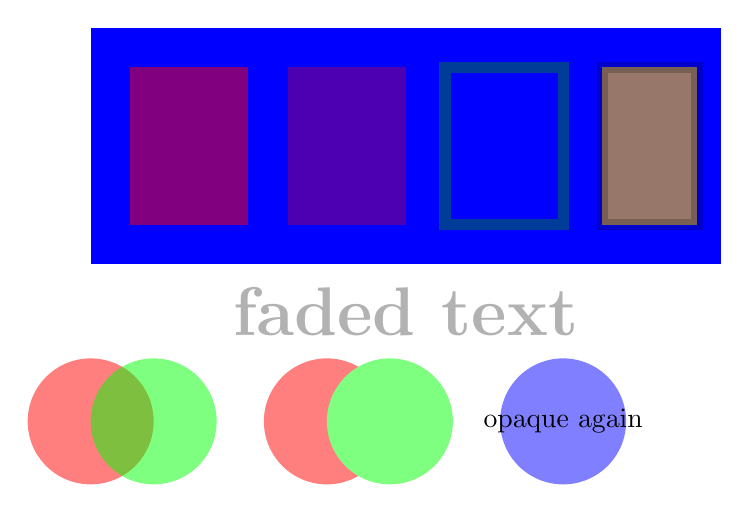
\begin{tikzpicture}[line width=4pt]
  \fill[blue] (0,0) rectangle (8,3);
  \fill[red, opacity=0.5] (0.5,0.5) rectangle (2,2.5);
  \fill[red, fill opacity=0.3] (2.5,0.5) rectangle (4,2.5);
  \draw[green!60!black, draw opacity=0.4] (4.5,0.5) rectangle (6,2.5);
  \filldraw[fill=yellow!80!red, draw=black, fill opacity=0.6, draw opacity=0.2] (6.5,0.5) rectangle (7.7,2.5);
  \node[text opacity=0.3, font=\Huge\bfseries, white] at (4,-0.6) {\color{black}faded text};
  \begin{scope}[opacity=0.5]
    \fill[red] (0,-2) circle (0.8);
    \fill[green] (0.8,-2) circle (0.8);
  \end{scope}
  \begin{scope}[transparency group, opacity=0.5]
    \fill[red] (3,-2) circle (0.8);
    \fill[green] (3.8,-2) circle (0.8);
  \end{scope}
  \fill[blue, opacity=0.5] (6,-2) circle (0.8);
  \node at (6,-2) {opaque again};
\end{tikzpicture}
\end{document}
